
\subsection{Answers}
\begin{table}[htb]%
\begin{center}%
\caption{Q15: What is the most difficult part of writing an MPI program?}%
\label{tab:Q15-ans}%
\begin{tabular}{l|l|r}%
\hline%
Choice & Abbrv. & \# Answers \\%
\hline%
Debugging & Debugging & 273 (32.5\%) \\%
Algorithm design & Algorithm & 204 (24.3\%) \\%
Performance tuning & Tuning & 152 (18.1\%) \\%
Domain decomposition & Decomposition & 98 (11.7\%) \\%
Implementation issue workaround & Workaround & 53 (6.3\%) \\%
Finding appropriate MPI routines & Finding MPI routines & 39 (4.6\%) \\%
other & - & 22 (2.6\%) \\%
\hline%
\multicolumn{2}{c}{total} & 841 \\%
\hline%
\end{tabular}%
\end{center}%
\end{table}%


\begin{figure}[htb]
\begin{center}
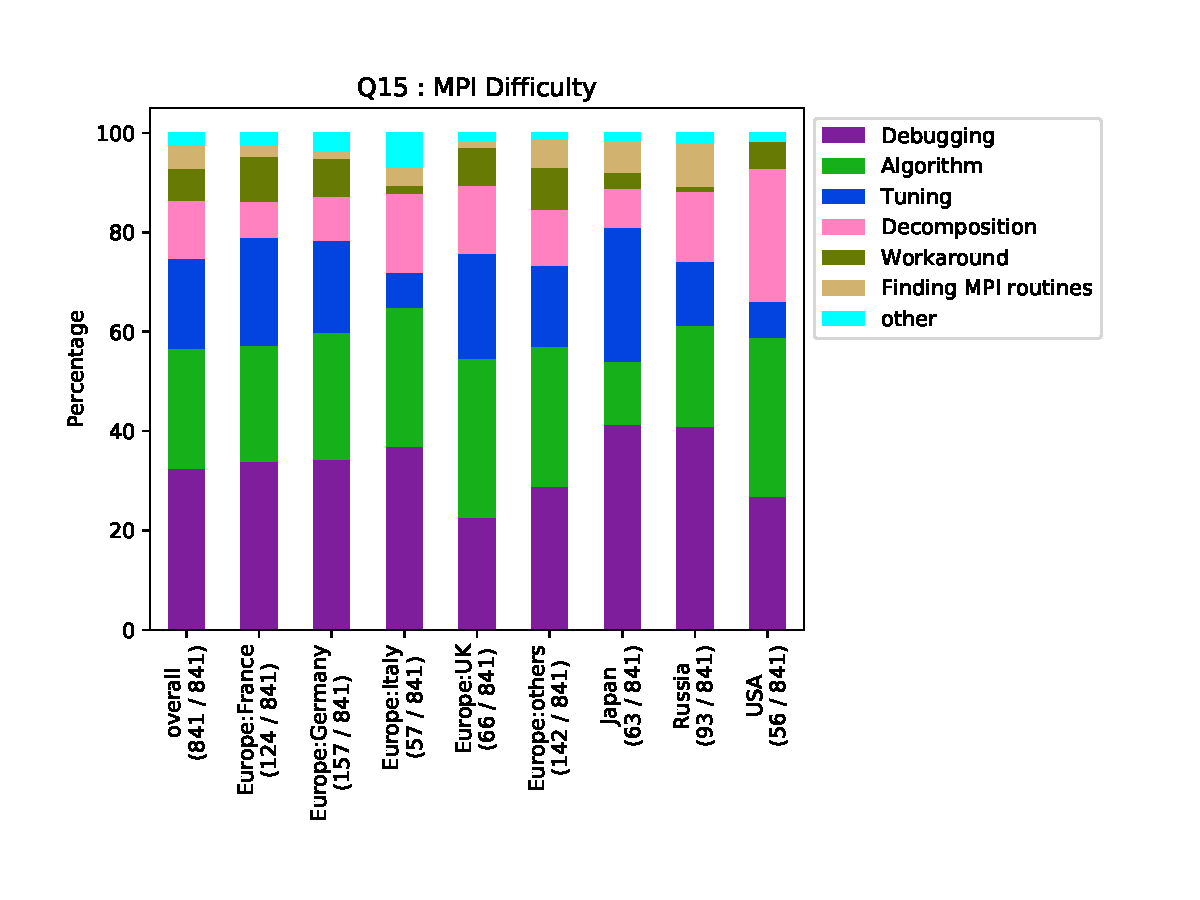
\includegraphics[width=10cm]{../pdfs/Q15.pdf}
\caption{Simple analysis: Q15}
\label{fig:Q15}
\end{center}
\end{figure}

Concerning the difficulty of writing MPI programs we can distinguish the issues
between (low-level) MPI related aspect (Debugging, performance tuning,
implementation issues, and finding routines) with higher-level issues close to
the program design (algorithm and domain decomposition). The former set of
issues is largely dominant with more than 60\% of the answers. This outlines
that the difficulties of writing a correct program in MPI is more related to the
the programming model and the standard that the design of the parallel program itself. 

This situation varies over country/region. In USA, the higher-level
issues dominate more than 50\% whilst lower-level issues dominate more
than 50\% in Japan. 